% ***************************************************************************************************
%
%	Szablon pracy magisterskiej dla Politechniki Wrocławskiej w wersji dwustronnej.
%	Autor:	Tomasz Strzałka
%
% ***************************************************************************************************

% Styl dwustronny z domyślną wielkością czcionki 10pt oraz oddzieloną stroną tytułową (titlepage).
% Domyślnie rodziały rozpoczynają się na stronie prawej (openright).
\documentclass{book}

% ***************************************************************************************************
% Ustawienia języka
% ***************************************************************************************************

% Podstawowe ustawienia języka, według którego formatowany będzie dokument
\usepackage[polish]{babel}

% Pakiet babel dla polskiego języka powoduje konflikt z pakietem amssymb.
% Polecenie '\lll' definiują oba pakiety - porządana jest druga definicja.
\let\lll\undefined

% W przypadku wielojęzykowości ustawia główny język dokumentu
\selectlanguage{polish}

% Kodowanie dokumentu
\usepackage[utf8]{inputenc}


% Dowolny rozmiar czcionek, kodowanie znaków
\usepackage{lmodern}


% Polskie wcięcia akapitów
\usepackage{indentfirst}

% Polskie łamanie wyrazów
\usepackage[plmath]{polski}

% Przecinek w wyrażeniach matematycznych zamiast kropki
\usepackage{icomma}

% Polskie formatowanie typograficzne
\frenchspacing

% Zapewnia liczne usprawnienia wyświetlania i organizacji matematycznych formuł. 
\usepackage{amsmath}

% Wprowadza rozszerzony zestaw symboli m.in. \leadsto
\usepackage{amssymb}

% Dodatkowa, ,,kręcona'' czcionka matematyczna
\usepackage{mathrsfs}

% Dodatkowe wsparcie dla środowiska mathbb, które nie wspiera domyślnie cyfr (\mathbb{})
\usepackage{bbold}

% Fixes/improves amsmath
\usepackage{mathtools}


% ***************************************************************************************************
% Kolory  
% ***************************************************************************************************

% Umożliwia kolorowanie poszczególnych komórek tabeli
\usepackage[table]{xcolor}% http://ctan.org/pkg/

% Umożliwia łatwą zmianę koloru linii w tabeli
\usepackage{tabu}

% Umożliwia rozszerzoną kontrolę nad kolorami.
\usepackage{xcolor}

% Definicje kolorów
\definecolor{lgray}{HTML}{9F9F9F}
\definecolor{dgray}{HTML}{5F5F5F}
% lgray				-	nazwa nowo zdefiniowanego koloru
% HTML				-	model kolorów
% CCCCCC			-	wartość koloru zgodna z modelem

% ***************************************************************************************************
% Algorytmy 
% ***************************************************************************************************

% Udostępnia środowisko do konstruowania pseudokodów
\usepackage[ruled,vlined,linesnumbered,longend,algochapter]{algorithm2e}
% ruled	- poziome kreski na początku i końcu algorytmu, podpis na górze oddzielony również kreską poziomą
% vlined - pionowe kreski łączące początek polecenia z jego końcem
% linesnumbered	- numerowanie kolejnych wierszy algorytmu
% longend - długie końcówki np. ifend, forend itd.
% algochapter - numeracja z rozdziałami

% Zamiana nazwy środowiska z domyślnej "Algorithm X" na "Pseudokod X"
\newenvironment{pseudokod}[1][htb]{
	\renewcommand{\algorithmcfname}{Pseudokod}
	\begin{algorithm}[#1]%
	}{
\end{algorithm}
}

% Zmiana rozmiaru komentarzy
\newcommand\algcomment[1]{
	\footnotesize{#1}
}

% Ustawienie zadanego stylu dla komentarzy
\SetCommentSty{algcomment}

% Wyśrodkowana tylda
\usepackage{textcomp}%
\newcommand{\textapprox}{\raisebox{0.5ex}{\texttildelow}}

% Listowanie kodów źródłowych
\usepackage{listings} 
\renewcommand{\lstlistingname}{Kod źródłowy} % Polska nazwa listingu

% Udostępnia środowisko do listowania kodów źródłowych z podświetleniem
\usepackage{minted}

% Definicje pecjalnych znaków, które nie są obsługiwane w środowisku listing
\lstset{literate=
	{ż}{{\.{z}}}1	{ź}{{\'{z}}}1
	{ć}{{\'{c}}}1	{ń}{{\'{n}}}1
	{ą}{{\c a}}1	{ś}{{\'{s}}}1
	{ł}{{\l}}1		{ę}{{\c{e}}}1
	{ó}{{\'{o}}}1	{á}{{\'a}}1
	{é}{{\'e}}1		{í}{{\'i}}1
	{ó}{{\'o}}1		{ú}{{\'u}}1
	{ù}{{\`u}}1		{Á}{{\'A}}1
	{É}{{\'E}}1		{Í}{{\'I}}1
	{Ó}{{\'O}}1		{Ú}{{\'U}}1
	{à}{{\`a}}1		{è}{{\'e}}1
	{ì}{{\`i}}1		{ò}{{\`o}}1
	{ò}{{\`o}}1		{À}{{\`A}}1
	{È}{{\'E}}1		{Ì}{{\`I}}1
	{Ò}{{\`O}}1		{Ò}{{\`O}}1
	{ä}{{\"a}}1		{ë}{{\"e}}1
	{ï}{{\"i}}1		{ö}{{\"o}}1
	{ü}{{\"u}}1		{Ä}{{\"A}}1
	{Ë}{{\"E}}1		{Ï}{{\"I}}1
	{Ö}{{\"O}}1		{Ü}{{\"U}}1
	{â}{{\^a}}1		{ê}{{\^e}}1
	{î}{{\^i}}1		{ô}{{\^o}}1
	{û}{{\^u}}1		{Â}{{\^A}}1
	{Ê}{{\^E}}1		{Î}{{\^I}}1
	{Ô}{{\^O}}1		{Û}{{\^U}}1
	{œ}{{\oe}}1		{Œ}{{\OE}}1
	{æ}{{\ae}}1		{Æ}{{\AE}}1
	{ß}{{\ss}}1		{ç}{{\c c}}1
	{Ç}{{\c C}}1	{ø}{{\o}}1
	{å}{{\r a}}1	{Å}{{\r A}}1
	{€}{{\EUR}}1	{£}{{\pounds}}1
}

% ***************************************************************************************************
% Marginesy 
% ***************************************************************************************************

% Ustawienia rozmiarów stron i ich marginesów
\usepackage[headheight=18pt, top=25mm, bottom=25mm, left=25mm, right=25mm]{geometry}
% headheight		-	wysokość tytułów
% top				-	margines górny
% bottom			-	margines dolny
% left				-	margines lewy
% right				-	margines prawy

% Usunięcie górnego marginesu dla środowisk
\makeatletter
\setlength\@fptop{0\p@}	
\makeatother

% ***************************************************************************************************
% Styl 
% ***************************************************************************************************

% Definiuje środowisko 'titlingpage', które zapewnia pełną kontrolę nad układem strony tytułowej.
\usepackage{titling}


% Umożliwia modyfikowanie stylu spisu treści
\usepackage{tocloft}	

\tocloftpagestyle{tableOfContentStyle}

% Definiowanie własnych stylów nagłówków i/lub stopek
\usepackage{fancyhdr}

% Domyślny styl dla pracy 
\fancypagestyle{custom}{
	\fancyhf{}									% wyczyść stopki i nagłówki
	\fancyhead[RO]{								% Prawy, nieparzysty nagłówek
		\hrulefill \hspace{16pt} \large Rozdział \thechapter
		\put(-472.1, 12.1){%
			\makebox(0,0)[l]{%
				
\includegraphics[width=0.05\textwidth]{pwr-logo}
			}
		}
		\put(-443,5.5){%
			\makebox(0,0)[l]{%
				\small Politechnika Wrocławska
			}
		}
	}
	\fancyhead[LE]{								% Lewy, parzysty nagłówek
		\large Rozdział \thechapter \hspace{16pt} \hrulefill 
		\put(-22, 12.1){%
			\makebox(0,0)[l]{%
				
\includegraphics[width=0.05\textwidth]{wppt-logo}
			}
		}
		\put(-210,5.5){%
			\makebox(0,0)[l]{%
				\small Wydział Podstawowych Problemów Techniki
			}
		}
	}
	\fancyfoot[LE,RO]{							% Stopki
		\thepage
	}
	\renewcommand{\headrulewidth}{0pt}			% Grubość linii w nagłówku
	\renewcommand{\footrulewidth}{0.2pt}		% Grubość linii w stopce
}


% Domyślny styl dla bibliografii
\fancypagestyle{bibliographyStyle}{
	\fancyhf{}									% wyczyść stopki i nagłówki
	\fancyhead[RO]{								% Prawy, nieparzysty nagłówek
		\hrulefill \hspace{16pt} \large Dodatek \thechapter
		\put(-472.1, 12.1){%
			\makebox(0,0)[l]{%
				
\includegraphics[width=0.05\textwidth]{pwr-logo}
			}
		}
		\put(-443,5.5){%
			\makebox(0,0)[l]{%
				\small Politechnika Wrocławska
			}
		}
	}
	\fancyhead[LE]{								% Lewy, parzysty nagłówek
		\large Bibliografia \hspace{16pt} \hrulefill 
		\put(-22, 12.1){%
			\makebox(0,0)[l]{%
				
\includegraphics[width=0.05\textwidth]{wppt-logo}
			}
		}
		\put(-210,5.5){%
			\makebox(0,0)[l]{%
				\small Wydział Podstawowych Problemów Techniki
			}
		}
	}
	\fancyfoot[LE,RO]{							% Stopki
		\thepage
	}
	\renewcommand{\headrulewidth}{0pt}			% Grubość linii w nagłówku
	\renewcommand{\footrulewidth}{0.2pt}		% Grubość linii w stopce
}

% Domyślny styl dla dodatków
\fancypagestyle{appendixStyle}{
	\fancyhf{}									% wyczyść stopki i nagłówki
	\fancyhead[RO]{								% Prawy, nieparzysty nagłówek
		\hrulefill \hspace{16pt} \large Dodatek \thechapter
		\put(-472.1, 12.1){%
			\makebox(0,0)[l]{%
				
\includegraphics[width=0.05\textwidth]{pwr-logo}
			}
		}
		\put(-443,5.5){%
			\makebox(0,0)[l]{%
				\small Politechnika Wrocławska
			}
		}
	}
	\fancyhead[LE]{								% Lewy, parzysty nagłówek
		\large Dodatek \thechapter \hspace{16pt} \hrulefill 
		\put(-22, 12.1){%
			\makebox(0,0)[l]{%
				
\includegraphics[width=0.05\textwidth]{wppt-logo}
			}
		}
		\put(-210,5.5){%
			\makebox(0,0)[l]{%
				\small Wydział Podstawowych Problemów Techniki
			}
		}
	}
	\fancyfoot[LE,RO]{							% Stopki
		\thepage
	}
	\renewcommand{\headrulewidth}{0pt}			% Grubość linii w nagłówku
	\renewcommand{\footrulewidth}{0.2pt}		% Grubość linii w stopce
}

% Osobny styl dla stron zaczynających rozdział/spis treści itd. (domyślnie formatowane jako "plain")
\fancypagestyle{chapterBeginStyle}{
	\fancyhf{}%
	\fancyfoot[LE,RO]{
		\thepage
	}
	\renewcommand{\headrulewidth}{0pt}
	\renewcommand{\footrulewidth}{0.2pt}
}

% Styl dla pozostałych stron spisu treści
\fancypagestyle{tableOfContentStyle}{
	\fancyhf{}%
	\fancyfoot[LE,RO]{
		\thepage
	}
	\renewcommand{\headrulewidth}{0pt}
	\renewcommand{\footrulewidth}{0.2pt}
}

% Formatowanie tytułów rozdziałów i/lub sekcji
\usepackage{titlesec}

% Formatowanie tytułów rozdziałów
\titleformat{\chapter}[hang]					% kształt
{
	\vspace{-10ex}
	\Huge
	\bfseries
}												% formatowanie tekstu modyfikowanego elementu
{}												% etykieta występująca przed tekstem modyfikowanego elementu, niewidoczna w spisie treści
{
	10pt
}												% odstęp formatowanego tytułu od lewego marginesu/etykiety
{
	\Huge
	\bfseries
}												% formatowanie elementów przed modyfikowanym tytułem
[
\vspace{2ex}
%\rule{\textwidth}{0.4pt}
%\vspace{-4ex}
]												% dodatkowe formatowanie stosowane poniżej modyfikowanego tytułu


% Formatowanie tytułów sekcji
\titleformat{\section}[hang]					% kształt
{
	\vspace{2ex}
%	\titlerule\vspace{1ex}
	\Large\bfseries
}												% formatowanie tekstu modyfikowanego elementu
{
	\thesection									% etykieta występująca przed tekstem modyfikowanego elementu, niewidoczna w spisie treści
}
{
	0pt
}												% odstęp formatowanego tytułu od lewego marginesu/etykiety
{
	\Large
	\bfseries
}												% formatowanie elementów przed modyfikowanym tytułem

% ***************************************************************************************************
% Linki
% ***************************************************************************************************

% Umożliwia wstawianie hiperłączy do dokumentu
\usepackage{hyperref}							% Aktywuje linki

\hypersetup{
	colorlinks	=	true,					% Koloruje tekst zamiast tworzyć ramki.
	linkcolor		=	blue,					% Kolory: referencji,
        citecolor		=	blue,					% cytowań,
	urlcolor		=	blue					% hiperlinków.
}

% Do stworzenia hiperłączy zostanie użyta ta sama (same) czcionka co dla reszty dokumentu
\urlstyle{same}




% ***************************************************************************************************
% Linki
% ***************************************************************************************************

% Umożliwia zdefiniowanie własnego stylu wyliczeniowego
\usepackage{enumitem}

% Nowa lista numerowana z trzema poziomami
\newlist{myitemize}{itemize}{3}

% Definicja wyglądu znacznika pierwszego poziomu
\setlist[myitemize,1]{
	label		=	\textbullet,
	leftmargin	=	4mm}

% Definicja wyglądu znacznika drugiego poziomu
\setlist[myitemize,2]{
	label		=	$\diamond$,
	leftmargin	=	8mm}

% Definicja wyglądu znacznika trzeciego poziomu
\setlist[myitemize,3]{
	label		=	$\diamond$,
	leftmargin	=	12mm
}

% ***************************************************************************************************
% Inne pakiety
% ***************************************************************************************************

% Dołączanie rysunków
\usepackage{graphicx}

% Figury i przypisy
\usepackage{caption}
\usepackage{subcaption}

% Umożliwia tworzenie przypisów wewnątrz środowisk
\usepackage{footnote}

% Umożliwia tworzenie struktur katalogów
\usepackage{dirtree}

% Rozciąganie komórek tabeli na wiele wierszy
\usepackage{multirow}

% Precyzyjne obliczenia szerokości/wysokości dowolnego fragmentu wygenerowanego przez LaTeX
\usepackage{calc}

% ***************************************************************************************************
% Matematyczne skróty
% ***************************************************************************************************

% Skrócony symbol liczb rzeczywistych
\newcommand{\RR}{\mathbb{R}}

% Skrócony symbol liczb naturalnych
\newcommand{\NN}{\mathbb{N}}

% Skrócony symbol liczb wymiernych
\newcommand{\QQ}{\mathbb{Q}}

% Skrócony symbol liczb całkowitych
\newcommand{\ZZ}{\mathbb{Z}}

% Skrócony symbol logicznej implikacji
\newcommand{\IMP}{\rightarrow}

% Skrócony symbol  logicznej równoważności
\newcommand{\IFF}{\leftrightarrow}

% ***************************************************************************************************
% Środowiska
% ***************************************************************************************************

% Środowisko do twierdzeń
\newtheorem{theorem}{Twierdzenie}[chapter]

% Środowisko do lematów
\newtheorem{lemma}{Lemat}[chapter]

% Środowisko do przykładów
\newtheorem{example}{Przykład}[chapter]

% Środowisko do wniosków
\newtheorem{corollary}{Wniosek}[chapter]

% Środowisko do definicji
\newtheorem{definition}{Definicja}[chapter]

% Środowisko do dowodów
\newenvironment{proof}{
	\par\noindent \textbf{Dowód.}
}{
\begin{flushright}
	\vspace*{-6mm}\mbox{$\square$}
\end{flushright}
}

% Środowisko do uwag
\newenvironment{remark}{
	\bigskip \par\noindent \small \textbf{Uwaga.}
}{
\begin{small}
	\vspace*{4mm}
\end{small}
}

% ***************************************************************************************************
% Słownik
% ***************************************************************************************************

% Prawidłowe dzielenie wyrazów
\hyphenation{wszy-stkich ko-lu-mnę każ-da od-leg-łość
	dzie-dzi-ny dzie-dzi-na rów-nych rów-ny
	pole-ga zmie-nna pa-ra-met-rów wzo-rem po-cho-dzi
	o-trzy-ma wte-dy wa-run-ko-wych lo-gicz-nie
	skreś-la-na skreś-la-ną cał-ko-wi-tych wzo-rów po-rzą-dek po-rząd-kiem
	przy-kład pod-zbio-rów po-mię-dzy re-pre-zen-to-wa-ne
	rów-no-waż-ne bi-blio-te-kach wy-pro-wa-dza ma-te-ria-łów
	prze-ka-za-nym skoń-czo-nym moż-esz na-tu-ral-na cią-gu tab-li-cy
	prze-ka-za-nej od-po-wied-nio}

% ***************************************************************************************************
% Dokument
% ***************************************************************************************************

\frontmatter

\begin{document}

	\begin{titlingpage}
		\vspace*{\fill}
		\begin{center}
			\begin{picture}(300,510)
				\put(11,520){\makebox(0,0)[l]{\large \textsc{Wydział Podstawowych Problemów Techniki}}}
				\put(11,500){\makebox(0,0)[l]{\large \textsc{Politechnika Wrocławska}}}
% Tytuł pracy
				\put(80,280){\Huge \textsc{Memory-hard Functions}}
% Autor pracy
				\put(90,200){\makebox(0,0)[l]{\large \textsc{Konrad Świerczyński}}}
				\put(90,180){\makebox(0,0)[l]{\large \textsc{Nr indeksu: 229818}}}

				%\put(200,100){\makebox(0,0)[l]{\large Praca inżynierska napisana}}
				%\put(200,80){\makebox(0,0)[l]{\large pod kierunkiem}}
				\put(200,80){\makebox(0,0)[l]{\large Promotor}}
% dane promotora
				\put(200,60){\makebox(0,0)[l]{\large dr Filip Zagórski}}
				
				\put(115,-70){
\includegraphics[width=0.15\textwidth]{pwr}}
				\put(106,-80){\makebox(0,0)[bl]{\large \textsc{Wrocław 2019}}}
			\end{picture}
		\end{center}	
		\vspace*{\fill}
	\end{titlingpage}
	
        \cleardoublepage
		
	\pagenumbering{Roman}
	\pagestyle{tableOfContentStyle}
	\tableofcontents
	\cleardoublepage
		
	% ***************************************************************************************************
	% Wstęp
	% ***************************************************************************************************
	
	\pagestyle{custom}
	\mainmatter
	
	% ***************************************************************************************************
	% Rodziały
	% ***************************************************************************************************

	\chapter{Wstęp}
\thispagestyle{chapterBeginStyle}


Niniejsza praca swoim zakresem obejmuje kryptograficzne funkcje do przechowywania haseł typu \textit{memory-hard} zapewniającą wysokie bezpieczeństwo przechowywania haseł.
Celem pracy jest analiza bezpieczeństwa oraz implementacja funkcji tego typu, jaką jest RiffleScrambler \cite{rs}. Praca przedstawia także definicje opisu jakości takich funkcji oraz przedstawia porównanie RiffleScrambler do obecnych rozwiązań.

W rozdziale \ref{rozdzial1} przedstawiono motywację, formalne definicje oraz twierdzenia potrzebne po przeprowadzenia analizy bezpieczeństwa oraz porównywania funkcji \textit{memory-hard}.
Rozdział \ref{razdzial2} przedstawia opis algorytmów, analizę bezpieczeństwa i porównanie do istniejących rozwiązań.
Rozdział \ref{rozdzial3} opisuje wykonane prace implementacyjne oraz dokumentację interfejsu.
W rozdziale \ref{rozdzial4} przedstawiono wymagania oraz sposób uruchomienia implementacji.
\nameref{podsumowanie} zawiera podsumowanie ukończonych prac oraz uzyskanych wyników.


	\cleardoublepage

	\chapter{Analiza problemu}
\thispagestyle{chapterBeginStyle}
\label{rozdzial1}

\begin{definition}
	(\textit{Parallel/Sequential Graph Pebbling}). Niech $G = (V, E)$ będzie grafem skierowanym grafem acyklicznym i niech $T \subset V$ będzie podzbiorem wierzchołków do oetykietowania, nazywanym celem.
	Stanem etykietowania $G$ jest podzbiór $P_{i} \subset V$.
	Poprawnym etykietowaniem równoległym jest ciąg $P = (P_{0}, \dots , P_{t})$ stanów etykietowania $G$,
	gdzie $P_{0} = \emptyset $ oraz gdzie spełnione są warunki 1 oraz 2 poniżej.
	Etykietowanie sekwencyjne musi dodatkowo spełniać warunek 3.
	\begin{enumerate}
		\item Każdy wierzchołek z celu jest w pewnej konfigutracji oetykietowany (nie koniecznie wszytkie jednocześnie).
		$$ \forall x \in T \exists x \leq t : x \in P_{x} $$
		
		\item Oetykietować wierzchołek można tylko wtedy, gdy wyszyscy jego rodzice
		są oetykietowani w poprzenim kroku.
		$$ \forall i \in [t] : x \in (P_{i} \setminus P_{i-1}) \Rightarrow parents(x) \subset P_{i-1} $$
		
		\item W każdym kroku można oetykietować co najwyżej jeden wierzchołek.
		$$ \forall i \in [t]: | P_{i} \setminus P_{i-1} | \leq 1 $$
	\end{enumerate}
\end{definition}


\begin{proof}
	dowód trywialny
\end{proof}


	\cleardoublepage

	\chapter{Riffle Scrambler}
\thispagestyle{chapterBeginStyle}

RiffleScrambler \cite{rs} jest nową rodziną acyklicznych grafów skierowanych, której odpowiada funkcja \textit{memory-hard} z dostępem do pamięci niezależnym od hasła, jest więc to iMHF.
W funkcji tej, podobnie jak w Catenie, kolejność obliczeń zdefiniowana jest za pomocą grafu. 
Przewagą funkcji RiffleScrambler, jest to, że dla Cateny są dwa predefiniowane grayf \textit{bit-reversal} i \textit{double-butterfly}, natomiast dla funkcji RiffleScrambler, graf jest generowany na podstawie soli, tak jak w funkcji Ballon Hashing. Oznacza, to, że dla każda sól odpowiada (z dużym prawdopodobieństwem) innemu grafowi, co zwiększa odporność na ataki równoległe.
Jednocześnie RiffleScrambler zapewnia lepszą wydajność przy obliczaniu niż Ballon Hashing, ponieważ ma dużo mniejszy stopień wchodzący grafu, który jest równy 3, a ponieważ jest superkoncentratorem, osiąga kompromis między pamięcią, a czasem oraz ograniczenie dolne złożoności etykietowania równoległego takie same jak Catena.

\section{Budowa Grafu}

\subsection{Parametry}
Funkcja RiffleScrambler używa następujących parametrów:
\begin{itemize}
	\item $s$ - sól, używana do wygenerowania grafu $G$,
	
	\item $g$ - ilość pamięci potrzebnej do obliczeń, dla $G = (V, E)$ zbiór wierzchołków można przedstawić jako $V = V_{0} \cup V_{1} \cup \dots \cup V_{2 \lambda g}$, gdzie $|V_{i}| = 2^{g}$,
	
	\item $\lambda$ - liczba warstw grafu $G$, może być postrzegana jako liczba iteracji.
\end{itemize}

Sól używana jest do generowania liczb pseudolosowych, potrzebnych do zbudowania grafu.
Parametr $g$ określa ilość pamięci, jaką trzeba będzie wykorzystać podczas obliczania funkcji. Podczas obliczeń potrzebne jest $2^{g+1}$ komórek, gdzie każda przechowuje wynik kryptograficznej dunkcji skrótu.
Parametr $\lambda$ definiuje ile warstw będzie miał końcowy graf, co bezpośrednio wpływa na czas obliczania funkcji.


\subsection{Tworzenie Grafu Na Podstawie Permutacji}

Niech $HW(x)$ (ang. \textit{Hamming weight}) oznacza ilość jedynek w wyrazie binarnym $x$. Niech $\overline{x}$ oznacza negację wyrazu $x$, zatem $HW(\overline{x})$ oznacza liczbę zer w wyrazie $x$.

\begin{definition}
	Niech $B = (b_{0} \dots b_{n-1}) \in \{ 0, 1 \}^{n}$ będzie wyrazem binarny o długości n. Definiujemy rangę $r_{B}(i)$ $i$-tego bitu w $B$ jako
	$$ r_{B}(i) = | \{ j < i : b_{j} = b_{i} \} | .$$
\end{definition}

\begin{definition}
	(Riffle-Permutation). Niech $B - (b_{0} \dots b_{n - 1})$ będzie wyrazem binarnym o długości $n$. Permutacja $\pi$ indukowana przez $B$ zdefiniowana jest następująco

	$$
	\pi_{B}(i) =
	\begin{cases}
	r_{B}(i), & \text{if}\ b_{i} = 0 \\
	r_{B}(i) + HW(\overline{B}), & \text{if}\ b_{i} = 1 \\
	\end{cases}
	$$
	
	dla każdego $ 0 \leq i \leq n-1$.
	
\end{definition}

\begin{example}
	Niech $B = 11100100$, wtedy $r_{B}(0) = 0$, $r_{B}(1) = 1$, $r_{B}(2) = 2$,
	$r_{B}(3) = 0$, $r_{B}(4) = 1$, $r_{B}(5) = 3$, $r_{B}(6) = 2$, $r_{B}(7) = 3$.
	Mając rangi dla wszystkich pozycji, można utworzyć Riffle-Premutation indukowaną przez $B$ 
	$\pi_{B} = \bigl( \begin{smallmatrix}
	0 && 1 && 2 && 3 && 4 && 5 && 6 && 7 \\
	4 && 5 && 6 && 0 && 1 && 7 && 2 && 3
	\end{smallmatrix} \bigr) $ .
	Ilustracja tego przykładu widoczna poniżej. TODO link	
\end{example}

\begin{figure}[h]
	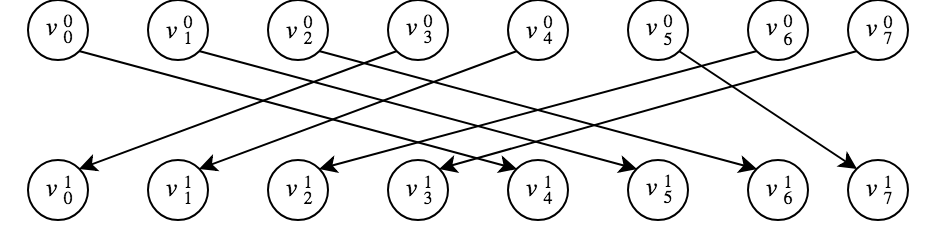
\includegraphics[width=\textwidth]{rp1.png}
	\centering
	\caption{Graf utowrzony z Riffle-Permutation indukowanej przez $B=11100100$.}
\end{figure}

\begin{definition}
	(N-Single-Layer-Riffle-Graph). Niech $V = V^{0} \cup V^{1}$, gdzie $V^{i} = \{ v_{0}^{i},\dots,v_{N-1}^{i} \}$ i niech $B$ będzie słowem binarnym długości $N$. Niech $\pi_{B}$ będzie Riffle-Permutaion indukowaną przez $B$.
	Graf N-Single-Layer-Riffle-Graph (dla parzystego N) zdefiniowany jest jako graf na wierzchołkach $V$ z następującymi krawędziami w zbiorze $E$:
	\begin{itemize}
		\item jedna krawędź: $v_{N-1}^{0} \rightarrow v_{0}^{1}$,
		
		\item $2(N - 1)$ krawędzi: $v_{i-1}^{j} \rightarrow v_{i}^{j}$, dla $i \in [N-1]$ oraz $j \in \{0, 1\}$,
		
		\item $N$ krawędzi: $v_{i}^{0} \rightarrow v_{\pi_{B}(i)}^{1}$, dla $i \in \{0,\dots,N -1\}$,
		
		\item $N$ krawędzi: $v_{i}^{0} \rightarrow v_{\pi_{\overline{B}}(i)}^{1}$, dla $i \in \{0,\dots,N -1\}$.
	\end{itemize}
\end{definition}

\begin{example}
	Kontynuując z danymi z poprzedniego przykładu TODO dodać link,
		$\pi_{\overline{B}} = \bigl( \begin{smallmatrix}
	0 && 1 && 2 && 3 && 4 && 5 && 6 && 7 \\
	0 && 1 && 2 && 4 && 5 && 3 && 6 && 7
	\end{smallmatrix} \bigr) $.
	 8-Single-Layer-Riffle-Graph ukazany jest na Rysynku TODO.
\end{example}

\begin{figure}[h]
	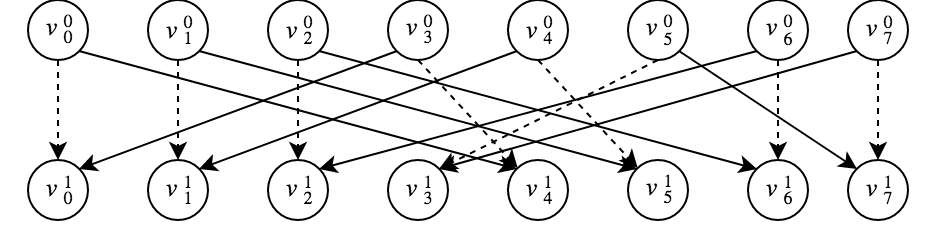
\includegraphics[width=\textwidth]{rp2.png}
	\centering
	\caption{8-Single-Layer-Riffle-Graph dla $B=11100100$ (krawędź $(v_{7}^{0}, v_{0}^{1})$ oraz krawędzie poziome zostały pominięte). Krawędzie dla permutacji $\pi_{B}$ oznaczone są linią ciągłą, a krawędzie dla permutacji $\pi_{\overline{B}}$ oznaczone są linią przerywaną.}
\end{figure}

Od teraz zakładamy, że $N = 2^{g}$.

\begin{definition}
	(N-Double-Riffle-Graph). Niech $V$ oznacza zbiór wierzchołków, a $E$ zbiór krawędzi grafu $G =(V, E)$. Niech $B_{0},\dots,B_{g-1}$ będą wyrazami binarnymi o długości $2^{g}$ każdy.
	N-Double-riffle-Graph jest otrzymywany poprzez ułożenie w stos $2g$ grafów, które spełniają warunki N-Single-Layer-Riffle-Graph. Otrzymany tak graf ma $(2g+1)2^{g}$ wierzchołków $ \{ v_{0}^{0}, \dots , v_{2^{g} - 1}^{0} \} \cup \dots \cup \{ v_{0}^{2g},\dots,v_{2^{g - 1}}^{2g} \} $,
	oraz następujące krawędzie:
	\begin{itemize}
		\item $(2g + 1)2^{g}$ krawędzi: $v_{i-1}^{j} \rightarrow v_{i}^{j}$ dla $i \in [2^{g}-1]$ i $j \in \{0,1,\dots,2^{g} \}$,
		
		\item $2g$ krawędzi: $v_{2^{g} - 1}^{j} \rightarrow v_{0}^{j+1}$ dla $j \in \{0,\dots,2g-1 \} $,
		
		\item $g2^{g}$ krawędzi: $v_{i}^{j-1} \rightarrow v_{\pi_{B_{j}}(i)}^{j}$, dla $i \in \{0,\dots,2^{g} -1\}$ i $j \in [g]$,
		
		\item $g2^{g}$ krawędzi: $v_{i}^{j-1} \rightarrow v_{\pi_{\overline{B}_{j}}(i)}^{j}$, dla $i \in \{0,\dots,2^{g} -1\}$ i $j \in [g]$,
	\end{itemize}
	oraz dla dolnych $g$ warstw, które są symetryczne względem warstwy $g$:
	\begin{itemize}
		\item $g2^{g}$ krawędzi: $v_{i}^{2g - j} \rightarrow v_{\pi_{B_{j}}^{-1}(i)}^{2g -j + 1}$, dla $i \in \{0,\dots,2^{g} -1\}$ i $j \in [g]$,

		\item $g2^{g}$ krawędzi: $v_{i}^{2g - j} \rightarrow v_{\pi_{\overline{B}_{j}}^{-1}(i)}^{2g - j + 1}$, dla $i \in \{0,\dots,2^{g} -1\}$ i $j \in [g]$,
	\end{itemize}

\end{definition}


\begin{definition}
	((N,$\lambda$)-Double-Riffle-Graph). Niech $G_{i}$, $i \in \{ 0,1,\dots,\lambda - 1\}$ będą N-Double-Riffle-Graph. Graf (N,$\lambda$)-Double-Riffle-Graph jest skonstruowany poprzez złączenie wyjść grafu $G_{i}$ do dopowiadających wejść grafu $G_{i+1}$, $i \in \{ 0, 1, \dots, \lambda - 2\}$.
\end{definition}

\subsection{Śledzienie Trajektorii}
Graf jest generowany za pomocą permutacji pseudolosowej $\sigma$.
Ponieważ do generowania grafu potrzebne jest $g$ słów binarnych o długości $2^{g}$, a permutacje zawierają $2^{g}$ elementów, gdzie każdy ma maksymalnie $g$ bitów znaczących, trzeba przekształcić permutację tak, aby otrzymać pożądane dane.
Ta procedura nazwana jest śledzeniem trajektorii (ang. \textit{trace trajectories}).
Niech $B$ będzie macierzą binarną o rozmiarze $2^{g} \times g$, gdzie $j$-ta kolumna jest binarną postacią $\sigma(j) \in [2^{g}-1]$. Macierz $\mathfrak{B} = (\mathfrak{B}_{0},\dots,\mathfrak{B}_{g-1})$ oznaczać będzie transpozycję macierzy $B$, a więc macierz o potrzebnym do generacji grafu rozmiarze $g \times 2^{g}$.


\section{Tworzenie Permutacji}

\subsection{Talia Kart Jako Permutacja}
Początkową częścią funkcji $\mathbf{RiffleScrambler}$ jest generowanie permutacji na podstawie soli. Do utworzenia takiej permutacji używany jest algorytm $\mathbf{InverseRiffleShuffle}$, który imituje odwrócenie tasowania kart do gry.
Podczas tasowania talia kart dzielona jest na dwie części.
Podział odbywa się poprzez wybranie karty w środku talii, karty które są przed wybraną kartą tworzą pierwszą część, a pozostałe tworzą drugą część.
Następnie te dwie części są ze sobą łączone w jeden stos poprzez losowe umieszczanie karty z góry pierwszej lub drugiej części na stosie.
Można zauważyć, że kolejność kart wśród stosu z którego pochodzą nie zmienia się, lecz między kolejne karty z jednego stosu mogą wejść karty z drugiego.

W celu wygenerowania permutacji $N$ elementów, myślimy o tych elementach jako o kartach, a o permutacji, jako o pewnej ich kolejności.
Krok odwrotnego sortowania wygląda następująco.

Dla każdej karty w talii losowany jest jeden bit, 0 lub 1. Wszystkie karty, dla których wylosowano 1 wyciągamy, zachowując ich kolejność i układamy na stos. Następnie umieszczamy ten stos na stosie kart, dla których wylosowano zera.

Dla każdego takiego kroku, dla każdej karty zapisywana jest informacja jaki bit został dla niej wylosowany. Zatem po $n$ krokach, każda karta ma przypisany ciąg binarny długości $n$.
Kończymy, kiedy talia kart jet dobrze posortowana, czyli kiedy każdej karcie przypisano unikalny ciąg binarny. Nowa kolejność elementów oznacza wygenerowaną permutację.

Można zauważyć, że liczba kroków tasowania $N$ kart na pewno nie będzie mniejsza od $\log{N}$, bo potrzebujemy $\lceil \log{N} \rceil$ bitów, aby każdej karcie przyporządkować inny ciąg binarny.

Algorytm $InverseRiffleShuffle$ będzie mógł się zakończyć, kiedy każdy element będzie posiadał różny ciąg binarny. Średnio oznacza to $2 \log{N}$ kroków \cite{rs}.

\subsection{Algorytm}
Razem z prezentacją funkcji $\mathbf{RiffleScrambler}$ zaproponowany został algorytm generowania permutacji \cite[algorym 1]{rs}, który sprawdzał warunek końca w czasie $O(n^2)$ oraz potrzebował $O(n^2)$ komórek pamięci, gdzie $n$ oznacza wielkość permutacji.

Pseudokod [IRS...] przedstawia algorytm sprawdzający warunek końca w czasie $O(n)$ korzystając z $O(n log{n})$ komórek pamięci.

Algorytm opiera się na sortowaniu pozycyjnym \textit{radix sort}, gdzie jako pozycje sortowanych elementów podawane są losowane bity.
Permutowane elementy, trzymane są w tablicy, która jest sortowana po każdej iteracji dokładania kolejnego bitu. Dzięki temu sprawdzenie warunku końca odbywa się na posortowanej tablicy, którą wystarczy przejść sprawdzając czy każde dwa sąsiednie elementy są różne, co wykonywane jest w czasie liniowym.

\section{Algorytm}

Procedurę $\mathbf{RiffleScrambler}(pwd, s, g,\lambda)$ można z grubsza przedstawić następująco.

\begin{itemize}
	\item Dla podanej soli $s$ obliczana jest pseudolosowa permutacja $\sigma$ (używając algorytmu inverse Riffle Shuffle).
	
	\item Dla permutacji $\sigma$ tworzona jest macierz $\mathfrak{B} = \mathbf{TraceTrajectories}(B)$.
	
	\item Dla wyrazów binarnych $\mathfrak{B}_{0},\dots,\mathfrak{B}_{g-1}$ generowany jest graf $G$, który jest N-Double-Riffle-Graph. Przypomnijmy, $N = 2 ^ {g}$.
	
	\item Na grafie $G$ zainicjalizowanym wartością $pwd$, oblicze są wartości w ostatnim rzędzie ($v_{0}^{2g+1},\dots,v_{2^{g} - 1}^{2g + 1}$).
	
	\item Wartości z ostatniego rzędu przepisywane są do pierwszego, $v_{i}^{0} = v_{1}^{2g+1}$ dla $i \in \{ 0,\dots,2^{g}-1 \}$, a następnie znów oblicza się wartość ostatnich rzędów. Powtarzane jest $\lambda$ razy.
	
	\item Wartością końcową jest wartość w ostatnim wierzchołku, czyli w $v_{2^{g} - 1}^{2g}$.
\end{itemize}

\begin{example}
	(Generacja (8,1)-Double-Riffle-Graph).
	Skoro $N = 8$, to $g = 3$, ponieważ $N = 2^g$. $\lambda = 1$.
	Niech otrzymaną permutacją $\sigma$ będzie $\bigl( \begin{smallmatrix}
	0 && 1 && 2 && 3 && 4 && 5 && 6 && 7 \\
	5 && 4 && 6 && 3 && 2 && 7 && 0 && 1
	\end{smallmatrix} \bigr) $.
	Zatem binarna postać permutacji $B = \bigl( \begin{smallmatrix}
		1 && 1 && 1 && 0 && 0 && 1 && 0 && 0 \\
		0 && 0 && 1 && 1 && 1 && 1 && 0 && 0 \\
		1 && 0 && 0 && 1 && 0 && 1 && 0 && 1
	\end{smallmatrix} \bigr) $.
	Przeprowadzając śledzenie trajektorii, czyli transponując $B$ otrzymujemy
	$\mathfrak{B} = (\mathfrak{B_0}, \mathfrak{B_1}, \mathfrak{B_2})$, $\mathfrak{B} =\bigl( \begin{smallmatrix}
	1 && 1 && 1 && 0 && 0 && 1 && 0 && 0 \\
	0 && 0 && 1 && 1 && 1 && 1 && 0 && 0 \\
	1 && 0 && 0 && 1 && 0 && 1 && 0 && 1
	\end{smallmatrix} \bigr)^{T} $.
	
	Teraz należy obliczyć permutacje $\pi_{\mathfrak{B_0}},\pi_{\mathfrak{B_1}},\pi_{\mathfrak{B_2}}$:
	
	$$ \pi_{\mathfrak{B_0}}=\bigl( \begin{smallmatrix}
	0 && 1 && 2 && 3 && 4 && 5 && 6 && 7 \\
	4 && 5 && 6 && 0 && 1 && 7 && 2 && 3
	\end{smallmatrix} \bigr), $$
		$$ \pi_{\mathfrak{B_1}}=\bigl( \begin{smallmatrix}
	0 && 1 && 2 && 3 && 4 && 5 && 6 && 7 \\
	0 && 1 && 4 && 5 && 6 && 7 && 2 && 3
	\end{smallmatrix} \bigr), $$
		$$ \pi_{\mathfrak{B_2}}=\bigl( \begin{smallmatrix}
	0 && 1 && 2 && 3 && 4 && 5 && 6 && 7 \\
	4 && 0 && 1 && 5 && 2 && 6 && 3 && 7
	\end{smallmatrix} \bigr). $$
	
	Wygenerowany graf z krawędziami zależnymi od permutacji ukazany jest na ...
	Dodając do nie go krawędzie nie zależne od permutacji, otrzymujemy pełny graf (8,1)-Double-Riffle-Graph.
	
\end{example}


\begin{figure}
		\centering
		
\includegraphics[width=0.7\textwidth]{all_rs1.png}

		\caption{(8,1)-Double-Riffle-Graph (krawędzie niezależne od permutacji, czyli przekątne oraz krawędzie poziome, zostały pominięte). Krawędzie dla permutacji oznaczone są linią ciągłą, a krawędzie dla permutacji negacji oznaczone są linią przerywaną.}
\end{figure}

\begin{figure}
	\centering
	
\includegraphics[width=\textwidth]{total_rs.png}
	
	\caption{(8,1)-Double-Riffle-Graph ze wszystkimi krawędziami oraz oznaczeniem wejścia i wyjścia. Krawędzie dla permutacji oznaczone są linią ciągłą, krawędzie dla permutacji negacji oznaczone są linią przerywaną, a krawędzie nie zależne od permutacji oznaczone są liniami kropkowanymi}
\end{figure}


\begin{algorithm}[H]
	\caption{$\mathbf{RiffleScrambler}$}
	\SetAlgoLined
	\KwIn{s, g, pwd, $\lambda$, H - funckja sktóru}
	\KwOut{pwd hash}
	
	$\sigma = \mathbf{RiffleShuffle}(2^g, s)$ \;
	$G = (V,E) = \mathbf{GenGraph}(g, \sigma$) \;
	$v_0^0 = H(X)$ \;
	\For{$i = 1$ \KwTo $2^g-1$}{
		$v_i^0 = H(v_{i-1}^{0})$ \;
	}
	\For{$r = 1$ \KwTo $\lambda$}{
		\For{$j = 0$ \KwTo $2g$}{
			\For{$i = 0$ \KwTo $2^g-1$}{
				$v_i^{j+1} = 0$ \;
				\ForAll{$v \rightarrow v_i^{j+1} \in E$}{
					$v_i^{j+1} = H(v_i^{j+1}, v)$ \;
				}
			}	
		}
		\For{$i = 0$ \KwTo $2^g - 1$}{
			$v_i^0 = v_i^{2g+1}$ \;
		}
	}

	$hash = v_{2^g - 1}{2g}$ \;
	\Return $hash$ \;
\end{algorithm}










	\cleardoublepage
	
	\chapter{Implementacja}
\thispagestyle{chapterBeginStyle}
\label{rozdzial3}

Implementacja $\mathbf{RiffleScrambler}$ została napisana tak, aby spełniała wymagania konkursu na funkcję do przechowywania haseł \cite[PHC, ang \textit{Password Hashing Competition}]{phc}, który rozgrywał się w latach 2013 - 2015.

\section{Wymagania konkursu}
Wymagania konkursu PHC odnoszące się do implementacji:
\begin{itemize}
	\item implementacja powinna być napisana w języku C(++) w taki sposób, aby była przenośna,
	\item do implementacji powinny być dołączone instrukcje kompilacji (np. Makefile),
	\item interfejs powinien być dostępny do użycia w języku C, oraz powinien zapewniać funkcję z podaną poniżej sygnaturą,
	\item implementacja może używać biblioteki OpenSSL,
	\item do implementacji powinny zostać dołączone testy.
\end{itemize}

\begin{minted}[mathescape]{C}
// Interfejs zaproponowany w ogłoszeniu konkursu na funkcję do przechowywania haseł $\label{impl::phc}$
int PHS(void *out, size_t outlen, const void *in, size_t inlen,
	const void *salt, size_t saltlen, % unsigned int t_cost, unsigned int m_cost); 
\end{minted}

Na zwycięzce konkursu wybrano Argon2, a Catena, Lyra2 \cite{simplicio2015lyra2}, yescryt \cite{peslyak2014yescrypt} oraz Makwa \cite{pornin2015makwa} otrzymały specjalne wyróżnienie.

\section{Opis technologii}
Początkowa implementacja napisana została w języku Python 3.7, jednak ze względu na niską wydajność oraz nie spełnianie wymagań PHC napisana została ostatecznie w języku C++17, standard ISO/IEC 14882:2017 \cite{cpp17}.

W implementacji używana jest biblioteka OpenSSL \cite{openssl}.
Z podanej biblioteki użyto interfejsu EVP \cite{opensslevp}, który dostarcza podstawowe kryptograficzne funkcje skrótu takie jak SHA2, SHA3, blake2s czy ripemd160.


\section{Omówienie kodów źródłowych}
Omówiony zostanie interfejs funkcji $\mathbf{RiffleScrambler}$, który spełnia wymogi PHC oraz posiada dodatkowy wysokopoziomowy interfejs pozwalający na wygodne tworzenie aplikacji uwierzytelniającej.

Kompletne kody źródłowe znajdują się do płycie CD dołączonej do niniejszej pracy (patrz Dodatek \ref{plytaCD}).

\subsection{Wysokopoziomowy interfejs}
Wysokopoziomowy interfejs upraszcza użycie funkcji $\mathbf{RiffleScrambler}$ podczas pisania
programów na wyższym abstrakcji takich jak na przykład aplikacje uwierzytelniające.
Podobnie jak w implementacji zwycięzcy konkursu PHC (argon2)\cite{arogn2impl} w udostępnionych funkcjach znajdują się:
\begin{itemize}
	\item funkcja zwracająca wynik jako tekst ze znakami w systemie heksadecymalnym - linia \ref{impl::rs_str},
	\item funkcja zwracająca wynik jako wektor znaków w systemie heksadecymalnym - linia \ref{impl::rs_vec},
	\item funkcja zwracająca zakodowany wynik wraz z użytą solą oraz parametrami w celu łatwego przechowywania i łatwej weryfikacji, sól oraz hasło zakodowane są za pomocą base64 \cite{josefsson2006base16} - linia \ref{impl::rs_enc},
	\item funkcja weryfikująca poprawność podanego hasła dla zakodowanego wyniku - linia \ref{impl::rs_ver}.
\end{itemize}

Każda z podanych funkcji ma również sygnaturę, gdzie hasło i sól podawane są za pomocą typu \texttt{std::string}.

\begin{minted}[linenos=true, mathescape]{C++}

/**$\label{impl::rs_str}$
* Hashowanie hasła za pomocą RiffleScrambler 
* @param pwd Wskaźnik na hasło
* @param pwdlen_bytes Długość hasła w bajtach
* @param salt Wskaźnik na sól
* @param saltlen_bytes Długość soli w bajtach
* @param garlic Paremetr "g" oznaczający koszt pamięci
* @param depth Parametr "lambda" oznaczający koszt czasowy
* @param hash_func Nazwa kryptograficznej funkcji skrótu do użycia wewnątrz
* @return Hash hasła jako ciąg znaków w systemie szesnastkowym
*/
std::string riffle_scrambler(const void *const pwd, const size_t pwdlen_bytes,
const void *const salt, const size_t saltlen_bytes,
const uint64_t garlic, const uint64_t depth,
const std::string hash_func="sha256");


/** $\label{impl::rs_vec}$
* Hashowanie hasła za pomocą RiffleScrambler
* @param garlic Paremetr "g" oznaczający koszt pamięci
* @param depth Parametr "lambda" oznaczający koszt czasowy
* @param pwd Wskaźnik na hasło
* @param pwdlen_bytes Długość hasła w bajtach
* @param salt Wskaźnik na sól
* @param saltlen_bytes Długość soli w bajtach
* @param hash_func Nazwa kryptograficznej funkcji skrótu do użycia wewnątrz
* @return Hash hasła jako wektor znaków w systemie szesnastkowym
*/
std::vector<unsigned char> riffle_scrambler_hash_raw(const uint64_t garlic,
const uint64_t depth, const void *pwd, const size_t pwdlen_bytes,
const void *salt, const size_t saltlen_bytes, const std::string hash_func="sha256");


/**$\label{impl::rs_enc}$
* Hashowanie hasła za pomocą RiffleScrambler  
* kodowanie wyniku wraz z parametrami w jeden ciąg znaków
* @param garlic Paremetr "g" oznaczający koszt pamięci
* @param depth Parametr "lambda" oznaczający koszt czasowy
* @param pwd Wskaźnik na hasło
* @param pwdlen_bytes Długość hasła w bajtach
* @param salt Wskaźnik na sól
* @param saltlen_bytes Długość soli w bajtach
* @param hash_func Nazwa kryptograficznej funkcji skrótu do użycia wewnątrz
* @return Zakodowane parametry funkcji wraz z hashem hasła i solą
*/
std::string riffle_scrambler_encoded(const uint64_t garlic, const uint64_t depth,
const void *pwd, const size_t pwdlen_bytes,
const void *salt, const size_t saltlen_bytes, const std::string hash_func="sha256");


/** $\label{impl::rs_ver}$
* Weryfikacja hasha hasła z hashem zakodowanym hashem dla zakodowanych parametrów i soli
* @param encoded Zakodowane parametry wraz z hashem i solą
* @param pwd Wskaźnik na hasło
* @param pwd_len Długość hasła w bajtach
* @return true jeśli hashe są równe, false w przeciwny przypadku
*/
bool riffle_scrambler_verify(const std::string encoded, const void *pwd, const size_t pwd_len);


\end{minted}

\subsection{Niskopoziomowy interfejs}
Implementacja jest zgodna z interfejsem zaproponowanym przez PHC.
\begin{minted}[linenos=true, mathescape]{C++}
/**
* Hashowanie hasła za pomocą RiffleScrambler, wynik zwracany jest do zmiennej @hash
* @param pwd Wskaźnik na hasło
* @param pwdlen_bytes Rozmiar hasła w bajtach
* @param salt Wskaźnika na sól
* @param saltlen_bytes Rozmiar soli w bajtach
* @param t_cost Parametr "lambda" oznaczający ilość iteracji
* @param m_cost Parametr "g" oznaczający koszt rozmiar używanej pamięci
* @param hash Bufor do którego będzie zapisany hash hasła
* @param hashlen Rozmiar bufora, oznacza ile bajtów z hasha hasła ma zostać zapisane
* @return RIFFLE_SCRAMBLER_OK jeśli obliczenia zakończyły się pomyślnie, kod błędu w przeciwnym przypadku
*/
int riffle_scrambler(void *hash, const size_t hashlen, const void *pwd, const size_t pwdlen_bytes,
const void *salt, const size_t saltlen_bytes, const uint64_t t_cost, const uint64_t m_cost);
\end{minted}


\section{Parametry}
Funkcja przyjmuje parametry opisane w poprzednim rozdziale \ref{rs::g}.
\begin{itemize}
	\item Parametr \texttt{garlic} oznacza $g$ z poprzedniego rozdziału, czyli długość rzędu, która wynosi $N = 2^{g}$.
	Definiuje to rozmiar pamięci, która jest potrzebny do wykonania obliczeń.
	Ponieważ w pamięci trzymane są wartości z dwóch rzędów grafu w jednej chwili, czyli dwóch rzędów po $2^g$ elementów, gdzie każda trzyma wynik wewnętrznej funkcji haszującej. Zatem zapotrzebowanie na pamięć wynosi $2^{g + 1} \times m$, gdzie $m$ oznacza rozmiar wyniku funkcji haszującej (np. dla SHA256 jest to 256 bitów, tak jak wskazuje nazwa).
	Na ogólne zużycie pamięci przez program w obecnej wersji wpływa też graf, który jest generowany na początku i trzymany przez czas działania programu. Przyjmuje wartość od $0$ do $2^{24} - 1$.
	
	\item Parametr \texttt{depth} oznacza ilość warstw grafu i w poprzednim rozdziale oznaczony był jako $\lambda$, przyjmuje wartość całkowitą od $1$ do $2^{64} - 1$.
	
	\item \texttt{pwd} oznacza hasło. Może być to wskaźnik na dane o długości od $0$ do $2^{32} -1$ bitów. Nie jest sprawdzana jakość hasła.
	Zapewnienie, że podane hasło jest wystarczające długie lub spełnia pewne warunki leży po stronie programu używającego funkcję $\mathbf{RiffleScrambler}$.
	\item Parametr \texttt{salt} dostarcza do programu sól kryptograficzną o długości od $0$ do $2^{32} - 1$ bitów. Powinna być ona losowa oraz inna dla każdego z przechowywanych haseł, zalecaną długością soli jest co najmniej 16 bajtów \cite{PHC2013}.
	
	\item Parametr \texttt{hash\_func} określa funkcję hashującą, która ma być użyta wewnątrz $\mathbf{RiffleScrambler}$. Dostępne są następujące funkcje: sha224, sha256, sha384, sha512, ripemd160, blake2s256, blake2s512 oraz do celów testowych sha1, md5, mdc2.
\end{itemize}

Ważny jest dobór parametrów \texttt{garlic} ($g$) oraz \texttt{depth} ($\lambda$), ponieważ to od nich zależy bezpieczeństwo przechowywanych haseł. Zalecanymi parametrami, podobnie jak dla Argon2, jest $\texttt{garlic}=12$ oraz $\texttt{depth}=4$ zapewniające dostateczne bezpieczeństwo oraz racjonalny czas obliczeń. Oznacza to użycie pamięci wynoszące $16$ MiB, co jest wyższą wartością niż rozmiar pamięci podręcznej na poziomie L-1 oraz L-2 dla większości procesorów, a zazwyczaj nawet większa od całkowitej pamięci podręcznej, co wymusza kosztowne sięganie do pamięci RAM. 

\section{Uwidacznianie się własności \textit{memory-hard}}
Implementacja została zbadana pod kontem wydajności w zależności od podawanych parametrów.
Na podstawie wyników można zaobserwować, jak uwidacznia się własność \textit{memory-hard}.

Na wykresie \ref{impl::b2} widać, że zużycie pamięci rośnie wykładniczo od wartości parametru $g$.
Ponieważ zapotrzebowanie na pamięć rośnie, procentowo mniej elementów mieści się w pamięci podręcznej.

Dobrze odwzorowuje to wykres \ref{impl::b1}. Oprócz sytuacji dla $g < 7$, którą ciężko wyjaśnić, a więc biorąc pod uwagę wartości dla $g \geq 7$, liczba odwołań do danych, które nie znajdowały się w pamięci podręcznej (ang. \textit{chache misses}) zaczyna rosnąć od pewnego momentu.
Pierwszy wzrost ma miejsce dla $g = 10$, co odpowiada zapotrzebowaniu na pamięć ok. $1$ MiB. Biorąc pod uwagę, że pamięć podręczna obsługuje również inne procesy, w tym program monitorujący, można wnioskować, że liczba odczytów z pamięci RAM zaczyna być procentowo coraz większa od momentu, gdy zapotrzebowanie na pamięć dorównuje ilości pamięci podręcznej (procesor na maszynie testowej wyposażony był w $3$ MiB pamięci podręcznej).

Kontynuując to rozważanie, skoro liczba wolnych odczytów zaczyna przeważać dla dużych $g$, to czas obliczenia pojedynczego wierzchołka w grafie powinien się zwiększać. Tak właśnie się dzieje, co obrazuje wykres \ref{impl::b5}, który ilustruje czas obliczania pojedynczego wierzchołka w zależności od parametru $g$.

Co za tym idzie, obliczając graf z taką samą liczbą wierzchołków, ale dla różnych parametrów $g$ (wyrównując ilość wierzchołków za pomocą parametru $\lambda$), czas obliczeń takich funkcji powinien być wyższy dla większych wartości $g$. Tą zależność wydaje się potwierdzać wykres \ref{impl::b6}.

Oznacza to, że koszt odwoływania się do pamięci ma wpływ na czas obliczeń, co ilustruje własność \textit{memory-hard}.


Wykres \ref{impl::b3} przedstawia wpływ na czas obliczeń $\mathbf{RiffleScrambler}$ parametru $g$, który jest wykładniczy, oraz parametry $\lambda$, który jest liniowy.


\begin{figure}
	\begin{subfigure}{0.5\textwidth}
		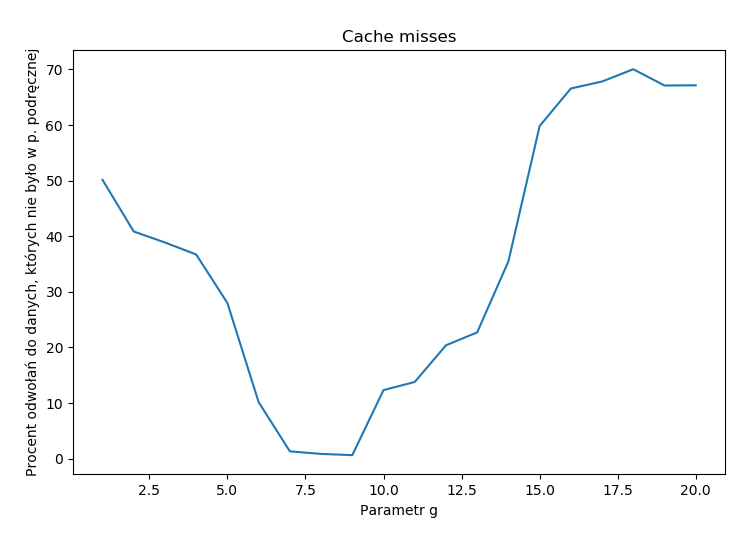
\includegraphics[width=\textwidth]{bench_1.png}
		\centering
		\caption{Wykresy liczby odczytów spoza pamięci podręcznej.}
		\label{impl::b1}
	\end{subfigure}
	\begin{subfigure}{0.5\textwidth}
		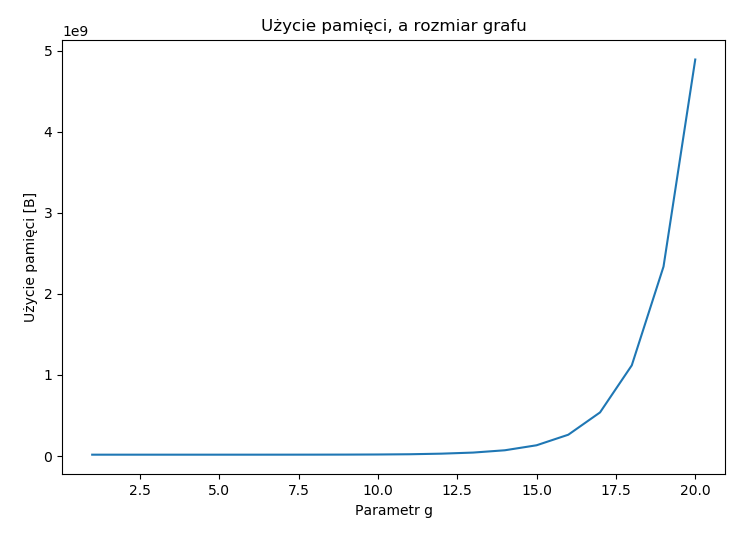
\includegraphics[width=\textwidth]{bench_2.png}
		\centering
		\caption{Wykresy zużycia pamięci przez $\mathbf{RiffleScrambler}$ w zależności od parametru $g$.}
		\label{impl::b2}
	\end{subfigure}
	\begin{subfigure}{0.5\textwidth}
		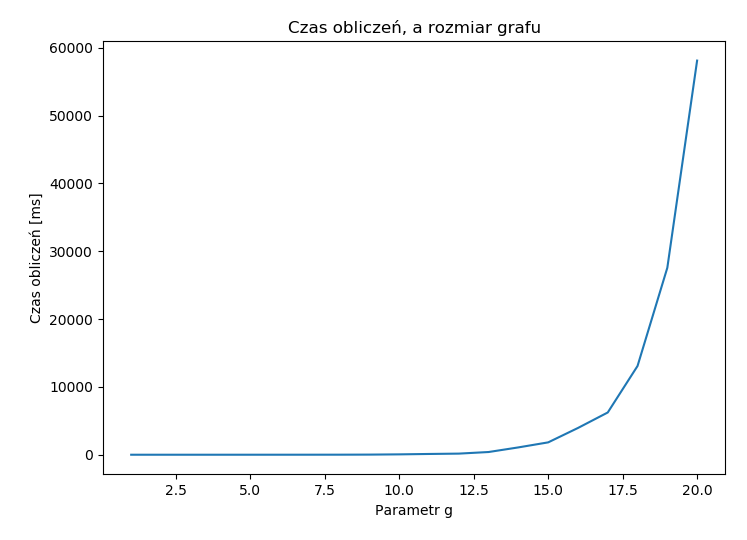
\includegraphics[width=\textwidth]{bench_3.png}
		\centering
		\caption{Wykres czasu obliczania $\mathbf{RiffleScrambler}$ w zależności od parametru $g$.}
		\label{impl::b3}
	\end{subfigure}
	\begin{subfigure}{0.5\textwidth}
		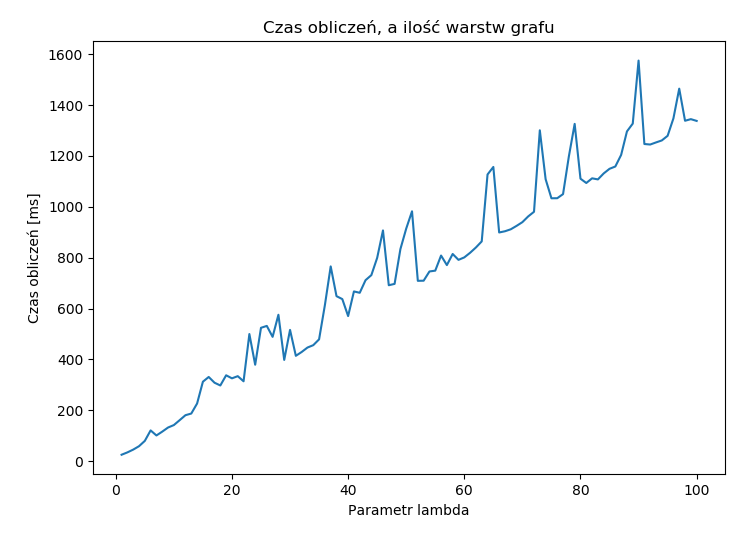
\includegraphics[width=\textwidth]{bench_4.png}
		\centering
		\caption{Wykres czasu obliczania $\mathbf{RiffleScrambler}$ w zależności od parametru $\lambda$.}
		\label{impl::b4}
	\end{subfigure}
		\begin{subfigure}{0.5\textwidth}
		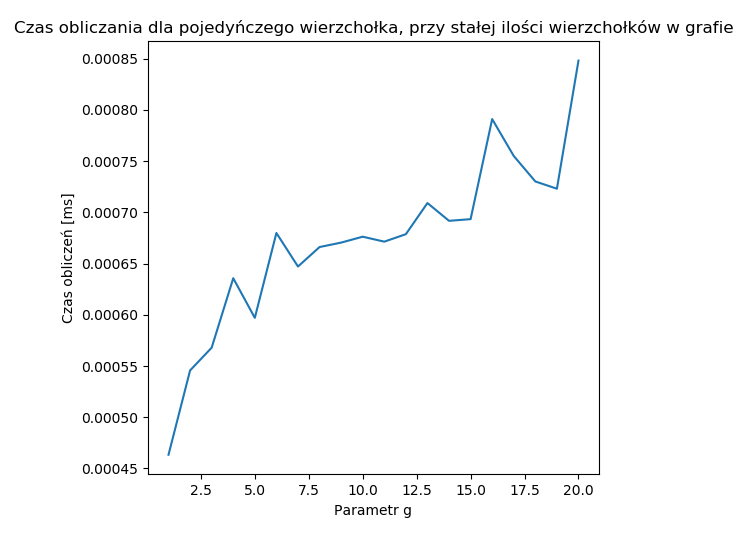
\includegraphics[width=\textwidth]{bench_5.png}
		\centering
		\caption{Wykres czasu obliczania $\mathbf{RiffleScrambler}$ w zależności od parametru $g$ dla stałej liczby wierzchołków w grafie.}
		\label{impl::b5}
	\end{subfigure}
	\begin{subfigure}{0.5\textwidth}
		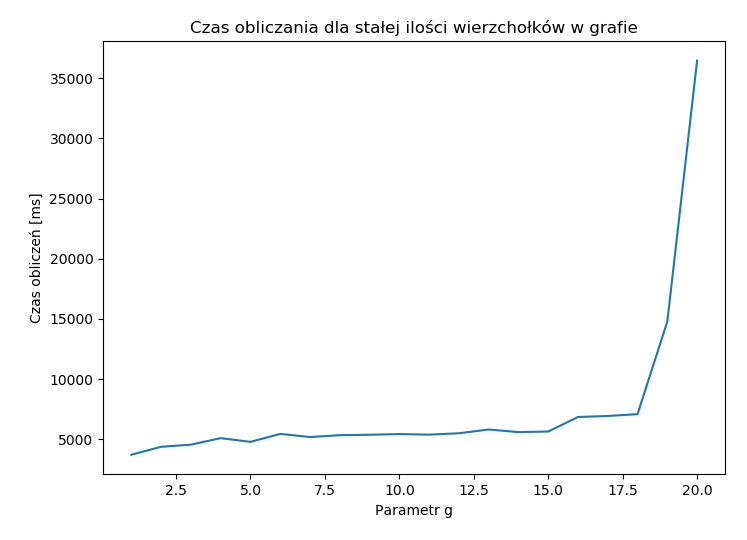
\includegraphics[width=\textwidth]{bench_6.png}
		\centering
		\caption{Średni czas obliczania jednego wierzchołka w zależności od parametru $g$ dla stałej liczby wierzchołków w grafie.}
		\label{impl::b6}
	\end{subfigure}

\end{figure}

\newpage
\section{RiffleScrambler w wierszu poleceń}
Do implementacji dołączony został też program \texttt{rs} uruchamiany z wiersza poleceń umożliwiający testowanie działania funkcji $\mathbf{RiffleScrambler}$ w łatwy sposób.
Aby wyświetlić instrukcje, jak używać tego programu należy wykonać polecenie \texttt{./rs -h} lub \texttt{./rs --help}.

\begin{lstlisting}
$ ./rs --help             
Password hashing memory-hard function
Usage:
RiffleScrambler  Password is read from stdin [OPTION...] [optional args]

-s, --salt arg   Salt for the given password
-w, --width arg  Width of the graph (default: 12)
-d, --depth arg  Number of stacks of the graph (default: 2)
-f, --func arg   Internal hash function (default: sha256)
-h, --help       Print help
\end{lstlisting}

Program przyjmuje parametry do uruchomienia funkcji $\mathbf{RiffleScrambler}$ w argumentach wywołania, natomiast hasło przyjmuje na standardowe wejście, ponieważ większość wierszy poleceń zapisuje historię wywołań programów i hasło podane jako argument wywołania mogłoby zostać zapisane w postaci jawnej.

Przykład użycia programu do obliczenia funkcji dla hasła \texttt{password}, soli \texttt{somesalt}, parametru g \texttt{16}, parametru $\lambda$ \texttt{2} używając \texttt{sha256} jako funkcji wewnętrznej.
\begin{lstlisting}[language=bash]
$ echo -n "password" | ./rs somesalt -w 16 -d 2 -f sha224
Graph width:	16
Graph depth:	2
Hash:       	166c88a5edfba7228fbf49a4bcd4cb2f01cc5fcdc850bf78c317a5c8
Encoded:    	$g=16$d=2$s=c29tZXNhbHQ=$f=sha224$h=MTY2Yzg4YTVlZGZiYTcyMjhmYmY0(...)
\end{lstlisting}

\section{Przykład użycia}
Wysokopoziomowy interfejs umożliwia uwierzytelnianie w wygodny sposób.
Zaprezentowany zostanie przykład użycia biblioteki \texttt{riffle} w aplikacji internetowej
podłączonej do bazy danych SQL. Aplikacja ta pozwala na zakładanie kont dla nowych użytkowników, oraz po zalogowaniu się na konto przez użytkownika, udostępnia użytkownikowi pewne zasoby.
Biblioteka \texttt{riffle} zostanie wykorzystana przy tworzeniu nowego konta, w celu obliczenia wartości funkcji $\mathbf{RiffleScrambler}$ dla hasła użytkownika, którą można bezpiecznie trzymać w bazie danych oraz później podczas uwierzytelniania w celu weryfikacji poprawności hasła.


Tabela użytkowników w bazie danych została utworzona następująco.
\begin{minted}[linenos=true]{SQL}
CREATE TABLE Users (
UserID int,
Login varchar(255),
HahsEncoded varchar(255),
Name varchar(255),)
);
\end{minted}

\begin{minted}[mathescape]{C++}
// importowanie interfejsu z biblioteki
#include <riffle/riffle_scrambler.h>


/**
* Funkcja zapisująca użytkownika w bazie danych
* @param login Login użytkownika
* @param password Hasło użytkownika (w postaci jawnej)
* @param name Imie użytkownika
* @param address Adres użytkownika
*/
void create_account(const std::string &login, const std::string &password,
	const std::string &name, const std::string &address) {
	
	// stowrzenie połączenia do bazy danych SQL
	const auto database_adapter = get_sql_database_adapter();

	// generowana jest losowa sól
	const std::string salt = generate_random_salt();
	// hasło użytkownika jest hashowane dla podanych parametrów oraz soli
	const std::string hash_encoded = riffle_scrambler_encoded(12, 4, password, salt);

	// jeden, bezpieczny do przechowywania
	// zawierający informacje o paramertach, soli oraz hashu tekst
	database_adapter.add_user(login, hash_encoded, name, address);
}


/**
* Funkcja do autoryzacji użytkownika na podstawie podanego hasła
* sprawdza, czy podane hasło jest takie samo, jak hasło podane przy tworzeniu konta,
* które zapisane jest w bazie danych
* @param login Login użytkownika
* @param password Hasło podane przez użytkownika
* @return true, jeśli podane przez użytkownika hasło jest poprawne,
* false w przeciwnym przypadku
*/
bool is_password_valid(const std::string &login, const std::string &password) {
	// stowrzenie połączenia do bazy danych SQL
	const auto database_adapter = get_sql_database_adapter();

	// pobranie wiersza z danymi użytkownika z bazy danych
	const auto user = database_adapter.get_user_by_login(login);

	// sprawdzenie czy wynik funkcji riffle_scrambler dla podanego przez użytkownika hasła
	// zgadza się z poprawnym hasłem dla podanego loginuxe
	return riffle_scrambler_verify(user.hash_encoded, password);
}
\end{minted}

To, co zasługuje na docenienie podczas używania biblioteki \texttt{riffle}, to konieczność poświęcenia tylko jednej kolumny w tabeli, aby uzyskać możliwość uwierzytelniania użytkownika za pomocą hasła. Nie trzeba przechowywać soli, ani parametrów funkcji, ponieważ zawarte są one w zakodowanej wartości. Oznacza to, że można zmienić dowolne parametry funkcji używane podczas tworzenia nowych kont oraz uwierzytelniać użytkowników z hasłami zapisanymi wcześniej bez konieczności rozróżniania z jakimi parametrami jaki użytkownik zakładał konto.

\newpage

\section{Testy}
Do implementacji zostały dołączone testy jednostkowe pisane przy wykorzystaniu biblioteki Catch2 \cite{catch}.

Testowane jest zewnętrzny interfejs oraz funkcje wewnętrzne.

Przykład uruchomienia testów.
\begin{lstlisting}
$ ./catch_test 
===============================================================================
All tests passed (740 assertions in 23 test cases)
\end{lstlisting}

Wymagania - cmake - make -openssl - kompilator

\section{Użycie implementacji}
\subsection{Wymagania}
Do kompilacji potrzebny jest kompilator języka C++ wspierający wersję C++17
\subsection{Biblioteka}
Kody biblioteki \texttt{riffle} znajdują się w katalogi \texttt{RiffleScrambler} zawierającym 
plik \texttt{CMakeLists.txt}.
W celu skompilowania biblioteki należy uruchomić polecenie \texttt{\$ cmake CMakeLists.txt} w katalogu \texttt{RiffleScrambler}, które wygeneruje plik \texttt{Makefile}. Następnie należy wykonać polecenie \texttt{\$ make}, które skompiluje kod biblioteki.


\subsection{Testy}



	\cleardoublepage
	
	\chapter{Podsumowanie}
\thispagestyle{chapterBeginStyle}
\label{podsumowanie}

W części teoretycznej niniejszej pracy udało się udowodnić dolne i górne ograniczenie na złożoność etykietowania grafu, ograniczenie dolne wynosi $\Omega(n^{1.5})$ i jest równe ograniczeniu górnemu Catena Dragonfly oraz Butterfly. Ograniczenie górne wynosi $O(n^{1,667})$, czyli jest wyższe, niż ograniczenie dla algorytmu Catena wynoszące $O(n^{1.625})$. Jednak wnioskując po podobieństwie tych grafów, bardzo prawdopodobne jest to, że istnieje lepsze ograniczenie górne, niż pokazane. Dlatego jest to możliwy kierunek rozwinięcia pracy.

W części praktycznej udało się zrealizować założenie o zachowaniu wymagań konkursu na funkcje do przechowywania haseł, ponadto zaproponowano nowy, wydajniejszy algorytm do generowania permutacji, który sprawdza poprawność permutacji w czasie liniowym, zamiast kwadratowego oraz cechuje się niższą złożonością pamięciową.
Stworzono również wysokopoziomowy interfejs, który jest dużą zaletą patrząc na aplikacje uwierzytelniające pisane w językach wysokopoziomowych.

Wydajność czasowa jest na dobrym poziomie, jednak wydajność pamięciowa mogłaby zostać poprawiona poprzez zmianę generowania struktury grafu, co okazało się podczas analizy pamięciowej gotowej implementacji. Zamiast generować od razu cały graf, który zajmuje stosunkowo dużo pamięci, można by trzymać jedynie obliczone obecnie używane krawędzie, a kolejne generować dopiero, gdy zajdzie potrzeba, co zmniejszyło by użycie pamięci.



	\cleardoublepage
	
	
	%%%%%%%%%%%%%%%%%%%%%%%%%%%%%%%%%%%%%%%%%%%%%%%%%%%%%%%%%%%%%%%%%%%%%%%%%%%%%%
	%%%%%%%%%%%%%%%%%%%%%%%%%%%%%%% BIBLIOGRAFIA %%%%%%%%%%%%%%%%%%%%%%%%%%%%%%%%%
	%%%%%%%%%%%%%%%%%%%%%%%%%%%%%%%%%%%%%%%%%%%%%%%%%%%%%%%%%%%%%%%%%%%%%%%%%%%%%%

	\pagestyle{bibliographyStyle}
	\bibliographystyle{plabbrv}
	\bibliography{literatura}
	\thispagestyle{chapterBeginStyle}
        \addcontentsline{toc}{chapter}{Bibliografia}

	\cleardoublepage
	
	%%%%%%%%%%%%%%%%%%%%%%%%%%%%%%%%%%%%%%%%%%%%%%%%%%%%%%%%%%%%%%%%%%%%%%%%%%%%%%
	%%%%%%%%%%%%%%%%%%%%%%%%%%%%%%%%% DODATKI %%%%%%%%%%%%%%%%%%%%%%%%%%%%%%%%%%%%
	%%%%%%%%%%%%%%%%%%%%%%%%%%%%%%%%%%%%%%%%%%%%%%%%%%%%%%%%%%%%%%%%%%%%%%%%%%%%%%
	
	\appendix
	\pagestyle{appendixStyle}
	
	\chapter{Zawartość płyty CD}
\thispagestyle{chapterBeginStyle}
\label{plytaCD}

W tym rozdziale należy krótko omówić zawartość dołączonej płyty CD.


	\cleardoublepage

\end{document}

